\documentclass[xcolor={dvipsnames}]{beamer}
\usepackage{color, colortbl}
\usepackage[ngerman,english]{babel}
\usepackage[T1]{fontenc}
\usepackage{CJKutf8} %japanese
\usepackage{lmodern}
\usepackage[compatibility=false]{caption}
\usepackage{subcaption}
\usepackage{tikz}
\usepackage{textgreek}
\usepackage{tabularx}
\usepackage{booktabs}
\usepackage{siunitx}
\usepackage{appendixnumberbeamer}
\usepackage[absolute,overlay]{textpos} %for positioning the logos where I want

\DeclareSIUnit\year{yr}

\mode<presentation>
{
  \usetheme{CambridgeUS}     
  \usecolortheme{lily} 
  \definecolor{beamer@violet}{rgb}{0.5,0.3,0.5} % changed this
  \setbeamercolor{structure}{fg=beamer@violet!70!cyan}
  \setbeamercolor{palette primary}{fg=black, bg=gray!30!white!50!cyan!20!}
  \setbeamercolor{palette secondary}{fg=black, bg=gray!30!white!30!cyan!40!}
  \setbeamercolor*{palette tertiary}{bg=gray!20!white!20!cyan!60!}
  
  \setbeamercolor{frametitle}{fg=cyan!60!white!40!,bg=cyan!80!black}
  \setbeamercolor{title}{fg=cyan!80!black}
  \setbeamercolor{normal text}{fg=black,bg=white}
  \setbeamercolor{alerted text}{fg=beamer@violet}
  \setbeamercolor{example text}{fg=beamer@violet!70!cyan}
  
  \usefonttheme{structureitalicserif} 
  \setbeamertemplate{navigation symbols}{}
  \setbeamertemplate{caption}[numbered]
}
\newcommand{\sidlogo}{
  \setlength{\TPHorizModule}{1pt}
  \setlength{\TPVertModule}{1pt}
   % textblock{}{x,y}: pos(x) = rightUpperCorner + (x * \TPHorizModule), pos(y) = leftUpperCorner - (y * \TPVertModule)
  \begin{textblock}{1}(323,12)
   
\includegraphics[width=40pt,height=26pt]{figures/SiD.jpeg}
  \end{textblock}
  } 
\newcommand{\ilclogo}{
  \setlength{\TPHorizModule}{1pt}
  \setlength{\TPVertModule}{1pt}
   % textblock{}{x,y}: pos(x) = rightUpperCorner + (x * \TPHorizModule), pos(y) = leftUpperCorner - (y * \TPVertModule)
  \begin{textblock}{1}(323,12)
   
\includegraphics[width=40pt,height=26pt]{figures/ILC.jpeg}
  \end{textblock}
} 
\newcommand{\atflogo}{
  \setlength{\TPHorizModule}{1pt}
  \setlength{\TPVertModule}{1pt}
   % textblock{}{x,y}: pos(x) = rightUpperCorner + (x * \TPHorizModule), pos(y) = leftUpperCorner - (y * \TPVertModule)
  \begin{textblock}{1}(323,12)
   
\includegraphics[width=40pt,height=26pt]{figures/ATF_logo.jpg}
  \end{textblock}
}
\newcommand{\flukalogo}{
  \setlength{\TPHorizModule}{1pt}
  \setlength{\TPVertModule}{1pt}
   % textblock{}{x,y}: pos(x) = rightUpperCorner + (x * \TPHorizModule), pos(y) = leftUpperCorner - (y * \TPVertModule)
  \begin{textblock}{1}(315,12)
   
\includegraphics[width=60pt,height=26pt]{figures/fluka_logo.png}
  \end{textblock}
} 
\newcommand{\rhullogo}{
  \setlength{\TPHorizModule}{1pt}
  \setlength{\TPVertModule}{1pt}
   % textblock{}{x,y}: pos(x) = rightUpperCorner + (x * \TPHorizModule), pos(y) = leftUpperCorner - (y * \TPVertModule)
  \begin{textblock}{1}(343,12)
   
\includegraphics[width=20pt,height=26pt]{figures/rhul_logo.png}
  \end{textblock}
}
\newcommand{\ejadelogo}{
  \setlength{\TPHorizModule}{1pt}
  \setlength{\TPVertModule}{1pt}
   % textblock{}{x,y}: pos(x) = rightUpperCorner + (x * \TPHorizModule), pos(y) = leftUpperCorner - (y * \TPVertModule)
  \begin{textblock}{1}(283,12)
   
\includegraphics[width=40pt,height=26pt]{figures/EJADE.jpeg}
  \end{textblock}
} 
\newcommand{\BDSsymbol}{
  \setlength{\TPHorizModule}{1pt}
  \setlength{\TPVertModule}{1pt}
   % textblock{}{x,y}: pos(x) = rightUpperCorner + (x * \TPHorizModule), pos(y) = leftUpperCorner - (y * \TPVertModule)
  \begin{textblock}{1}(0,39)
   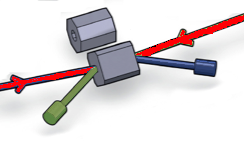
\includegraphics[width=60pt,height=40pt]{figures/Highlight_BDS.png}
  \end{textblock}
} 
\newcommand{\EXTsymbol}{
  \setlength{\TPHorizModule}{1pt}
  \setlength{\TPVertModule}{1pt}
   % textblock{}{x,y}: pos(x) = rightUpperCorner + (x * \TPHorizModule), pos(y) = leftUpperCorner - (y * \TPVertModule)
  \begin{textblock}{1}(0,39)
   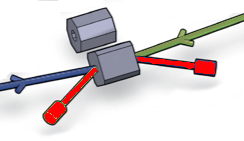
\includegraphics[width=60pt,height=40pt]{figures/Highlight_EXT.png}
  \end{textblock}
} 


\title[ILC \& Background Simulations]{\textbf{\alert{ECFA 2016} \\\LARGE Beam Backgrounds at the ILC}}
%\author{\textbf{Anne Sch\"utz}}
\author[Anne Sch\"utz]{\underline{Anne Sch\"utz} \inst{1}, Marcel Stanitzki \inst{1}, Jan Strube \inst{2}, Bruce Schumm \inst{3}, Christopher Milke \inst{3}, SiD collaboration\\
\vspace*{0.2cm}{\scriptsize In collaboration with:\\Benno List \inst{1}, Nuria Fuster Martinez \inst{4}, ATF staff \inst{5}, Glen White \inst{6}, L. Nevay \inst{7},\\J. Snuverink \inst{7}, S. Boogert \inst{7}}}

\institute[DESY]{\inst{1} DESY \inst{2} PNNL \inst{3} UCSC \inst{4} IFIC \inst{5} KEK \inst{6} SLAC \inst{7} RHUL}

%\institute{\textbf{KIT, DESY}}
\date{\textbf{04. May 2016}}

\titlegraphic{
\includegraphics[height=1.0cm]{figures/KIT.png}\hspace*{6cm}~%
   
\includegraphics[height=1.2cm]{figures/DESY_Logo.png}
}

\begin{document}

{
\usebackgroundtemplate{
 \tikz\node[opacity=0.1]{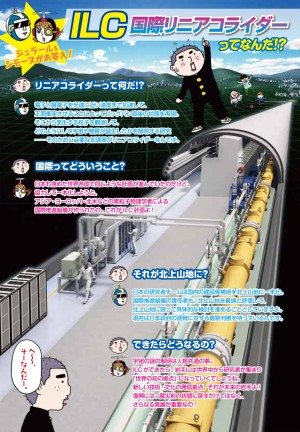
\includegraphics[width=\paperwidth]{figures/Iwatecomics.jpg}};
 % \tikz\node[opacity=0.2]{\centering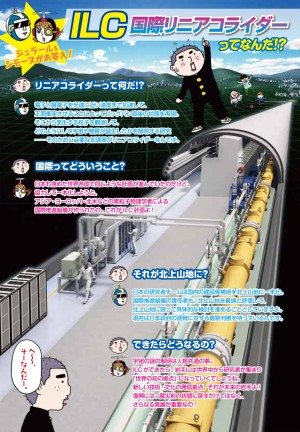
\includegraphics[height=\paperheight]{figures/Iwatecomics.jpg}};
 }
\begin{frame}
  \titlepage
\end{frame}
}

\begin{frame}{Table of contents}
  \tableofcontents
\end{frame}


\section{Background sources}
\begin{frame}{Background sources and simulation tools}
\ilclogo
The main sources of background:
\vspace*{0.5cm}
 \only<1>{
  \begin{itemize}
    \item Backgrounds from beam-beam interactions
    \begin{itemize}
      \item Pair background
      \item Bhabha scattering
      \item \textgamma \textgamma $\rightarrow$ hadrons
    \end{itemize}
    \item Neutrons from the beam dumps
    \item Background from the Final-Focus system
    \begin{itemize}
     \item Beam halo collimators
     \item Muons from spoilers
    \end{itemize}
  \end{itemize}
  }
  \only<2>{
  \begin{itemize}
    \item Backgrounds from beam-beam interactions
    \begin{itemize}
      \item \alert{Pair background - GuineaPig}
      \item \alert{Bhabha scattering - Whizard, Pythia}
      \item \alert{\textgamma \textgamma $\rightarrow$ hadrons - Whizard, Pythia}
    \end{itemize}
    \item Neutrons from the beam dumps
    \item Background from the Final-Focus system
    \begin{itemize}
     \item Beam halo collimators
     \item Muons from spoilers
    \end{itemize}
  \end{itemize}
  }
 \only<3>{
  \begin{itemize}
    \item Backgrounds from beam-beam interactions
    \begin{itemize}
      \item Pair background - GuineaPig
      \item Bhabha scattering - Whizard, Pythia
      \item \textgamma \textgamma $\rightarrow$ hadrons  - Whizard, Pythia
    \end{itemize}
    \item \alert{Neutrons from the beam dumps - FLUKA}
    \item Background from the Final-Focus system
    \begin{itemize}
     \item Beam halo collimators
     \item Muons from spoilers
    \end{itemize}
  \end{itemize}
  }
  \only<4>{
  \begin{itemize}
   \item Backgrounds from beam-beam interactions
    \begin{itemize}
      \item Pair background - GuineaPig
      \item Bhabha scattering - Whizard, Pythia
      \item \textgamma \textgamma $\rightarrow$ hadrons  - Whizard, Pythia
    \end{itemize}
    \item Neutrons from the beam dumps - FLUKA
    \item Background from the Final-Focus system
    \begin{itemize}
     \item \alert{Beam halo collimators - BDSIM}
     \item Muons from spoilers
    \end{itemize}
  \end{itemize}
  }
   \only<5>{
  \begin{itemize}
   \item Backgrounds from beam-beam interactions
    \begin{itemize}
      \item Pair background - GuineaPig
      \item Bhabha scattering - Whizard, Pythia
      \item \textgamma \textgamma $\rightarrow$ hadrons  - Whizard, Pythia
    \end{itemize}
    \item Neutrons from the beam dumps - FLUKA
    \item Background from the Final-Focus system
    \begin{itemize}
     \item Beam halo collimators - BDSIM
     \item \alert{Muons from spoilers - MUCARLO}
    \end{itemize}
  \end{itemize}
  }

\end{frame}

\section{Backgrounds from beam-beam interactions}

\begin{frame}
 \begin{center}
  \alert{\MakeUppercase{Backgrounds from beam-beam interactions}\\ \MakeUppercase{in the SiD detector}\\ 
  \vspace*{0.5cm}
  Pair background}\\
   \vspace*{0.3cm}
  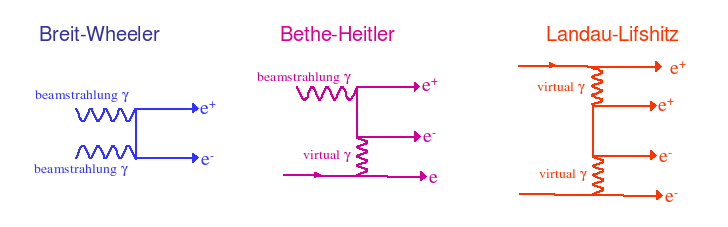
\includegraphics[height=0.3\textheight]{figures/beamstrahlung_processes.png}\\
  \vspace*{0.5cm}
  \alert{Bhabha scattering \& \textgamma \textgamma $\rightarrow$hadrons}\\
  \vspace*{0.3cm}
  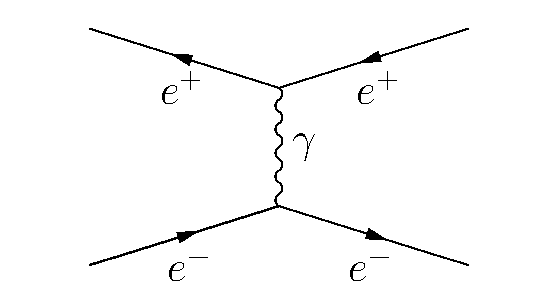
\includegraphics[height=0.2\textheight]{figures/bhabha_scattering.pdf} 
 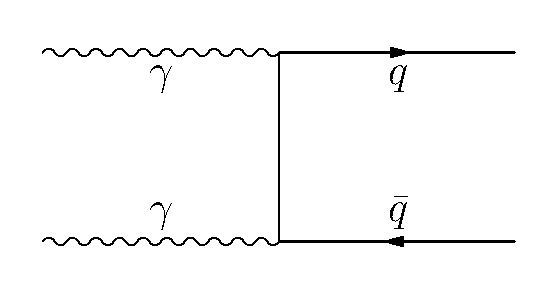
\includegraphics[height=0.2\textheight]{figures/gammagamma_hadrons.pdf}
  \end{center}
\end{frame}

\begin{frame}{Available files}
\sidlogo
 Generated background files are available for the community:
 \begin{itemize}
  \item Pair background: >3900 bunches for the ILC500 nominal beam parameters on the Grid
  \begin{itemize}
   \item at the IP: \cite{Grid}
   \item full detector simulations for different SiD geometries: \cite{Jan_Grid}
  \end{itemize}
  \item Bhabha scattering: $\sim$400 files (ILC500) for different SiD geometries on the Grid \cite{Jan_Grid}
  \item \textgamma\textgamma$\rightarrow$hadrons: $\sim$400 files (ILC500, +80e-/-30e+ and -80e-/+30e+) for different SiD geometries on the Grid \cite{Jan_Grid}
  \item Low cross section: (ILC500, +80e-/-30e+ and -80e-/+30e+) for different SiD geometries on the Grid \cite{Jan_Grid}
 \end{itemize}

\end{frame}


\begin{frame}{Ongoing studies}
\sidlogo
Example of ongoing studies on detector occupancies and hit time distributions:\\
\begin{block}{See also upcoming SiD note}
 \large``SiD concept design considerations prompted by high cross-section ILC processes''\\
 \small[Luc d`Hautuille, Christopher Milke, Bruce Schumm, Anne Sch\"utz, \\Marcel Stanitzki, Jan Strube]
\end{block}
\textit{\normalsize $\rightarrow$ Stay tuned!}
\end{frame}

\begin{frame}{Forward ECAL occupancies - all bkg}
\sidlogo
Occupancy and buffer depth studies in the Forward ECAL subdetector:\\
\flushright \tiny [Bruce Schumm, Christopher Milke, George Courcoubetis]\\
 \includegraphics[width=0.52\textwidth]{figures/zzfig_raw_occupancy.png}
\includegraphics[width=0.52\textwidth]{figures/zzfig_buffer_depth.png}\\
\flushleft \normalsize With a KPiX buffer depth of four, 1\% of the hits are lost\\ (because of full buffers).\\
With a buffer depth of eight, only 0.01\% of all hits are lost.
\end{frame}

\begin{frame}{Forward ECAL occupancies - all bkg}
\sidlogo
Dependency of the fractional loss of hits on the buffer depth and on the depth within the FCAL and the transverse distance from the beamline:\\
\flushright \tiny [Bruce Schumm, Christopher Milke, George Courcoubetis]\\
 \includegraphics[width=0.5\textwidth]{figures/zzfig_layer_buffer_depth_all.png}
\includegraphics[width=0.5\textwidth]{figures/zzfig_radial_buffer_depth_all.png}\\
\flushleft \normalsize No significant dependency on the layer depth is shown, but for smaller radii 7 or more buffers would reduce the fraction of lost hits to below \num{e-3}!\\ 
\tiny (The rise just before layer 20 is likely due to the increase in absorber thickness encountered at that depth in the calorimeter.)
\end{frame}

\begin{frame}{Vertex detector occupancies - Pair bkg}
\sidlogo
Comparison between different SiD geometries of the occupancy \underline{in layer 0}  of the vertex barrel and endcap as a function of phi and the radius:\\
\flushright \tiny [Bruce Schumm, Christopher Milke]\\
\includegraphics[width=0.52\textwidth]{figures/VradOccupancy_allGeoms_brl.png}
%\caption[Beamstrahlung processes]{VXD barrel layer 0 occupancies as a function of azimuthal angle.}
\includegraphics[width=0.52\textwidth]{figures/VradOccupancy_allGeoms_ecp.png}
%\caption[Beamstrahlung processes]{VXD endcap occupancies as a function of radius from the beamline.}
\flushleft \normalsize The SiD geometry with the anti-DiD or cutouts have comparable vertex occupancies, which are mainly lower than for the baseline design (sidloi3).\\
$\Rightarrow$All of the geometries show occupancies below \num{e-3} for all regions (except the innermost radii)!
\end{frame}

\begin{frame}{Vertex detector \& pair bkg time distributions}
\sidlogo
Distributions of the creation time and the hit time of the pair background particles hitting the SiD vertex detector:\\
\includegraphics[width=0.54\textwidth]{figures/creationtime_histo_SiVertexEndcapSiVertexBarrel.pdf}
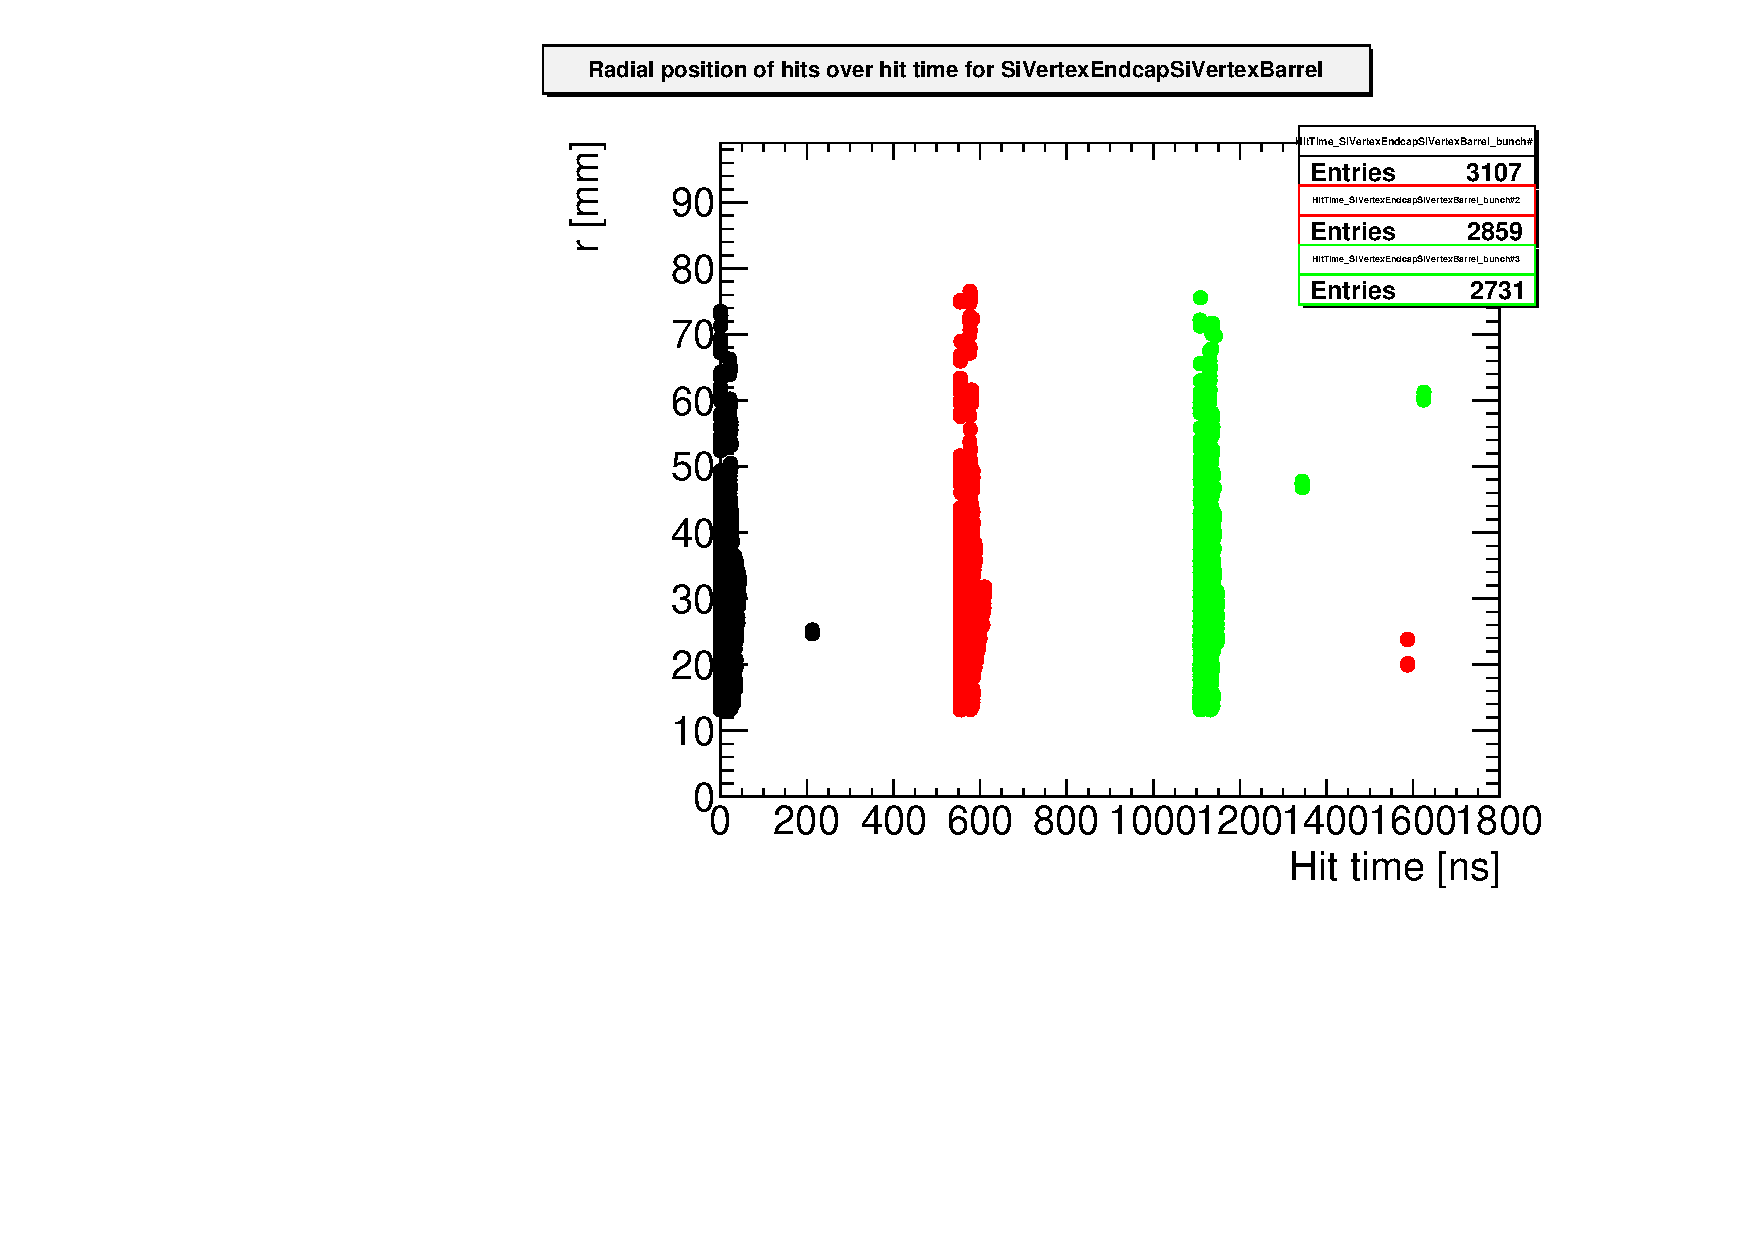
\includegraphics[width=0.54\textwidth]{figures/hittime_SiVertexEndcapSiVertexBarrel_IRrealign_3bunch.pdf}\\

\small 1312 bunches are accumulated for the left plot.\\
\normalsize The backscatter particles (backscattering from the SiD detector endcaps) are arriving up to several \textmu s late. 
\end{frame}

\begin{frame}{Particle origin of pair bkg particles hitting the vertex detector}
\sidlogo
 \begin{figure}
\begin{subfigure}[t]{0.49\textwidth}
\centering
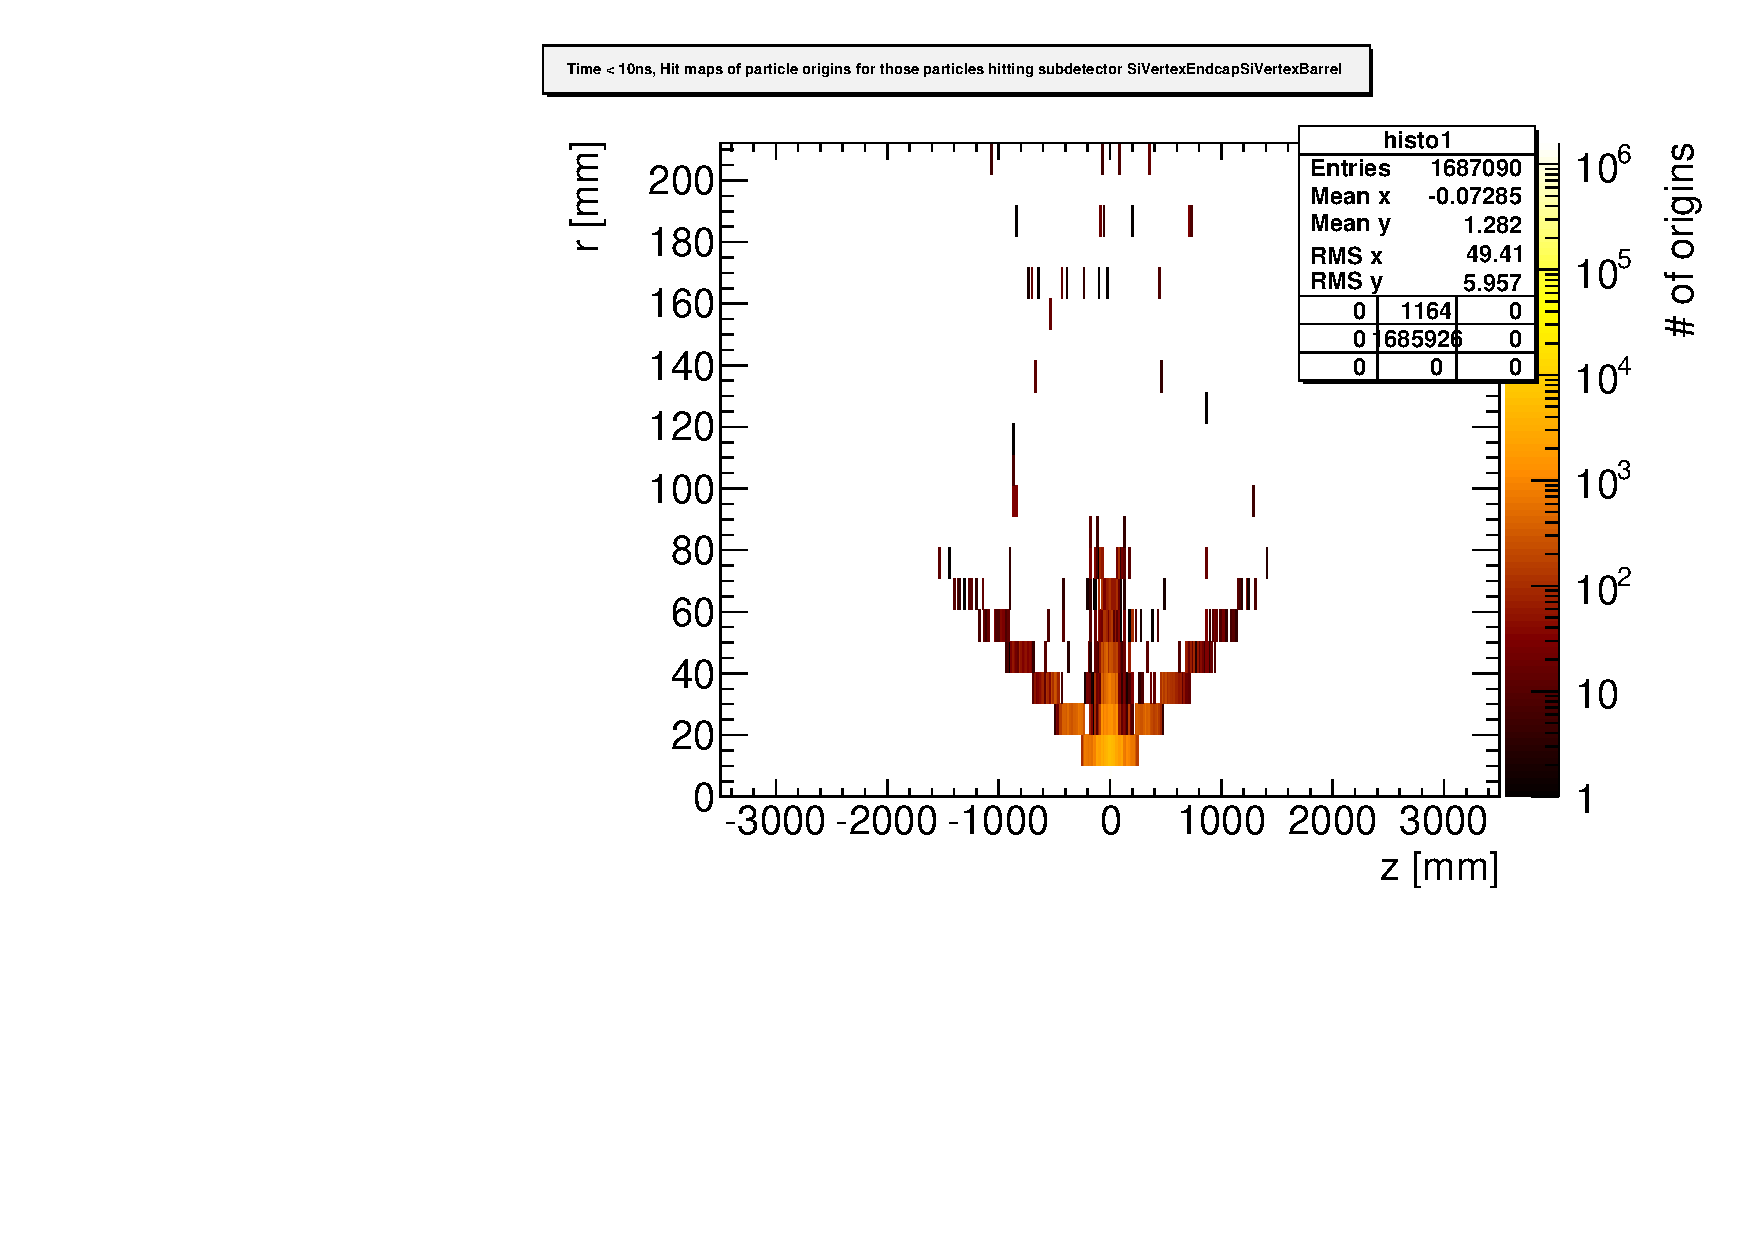
\includegraphics[width=\textwidth]{figures/hitmaps_particleorigins_time1_SiVertexEndcapSiVertexBarrel.pdf}
\caption{$[0\,ns;10\,ns]$.}
\end{subfigure}
\begin{subfigure}[t]{0.49\textwidth}
\centering
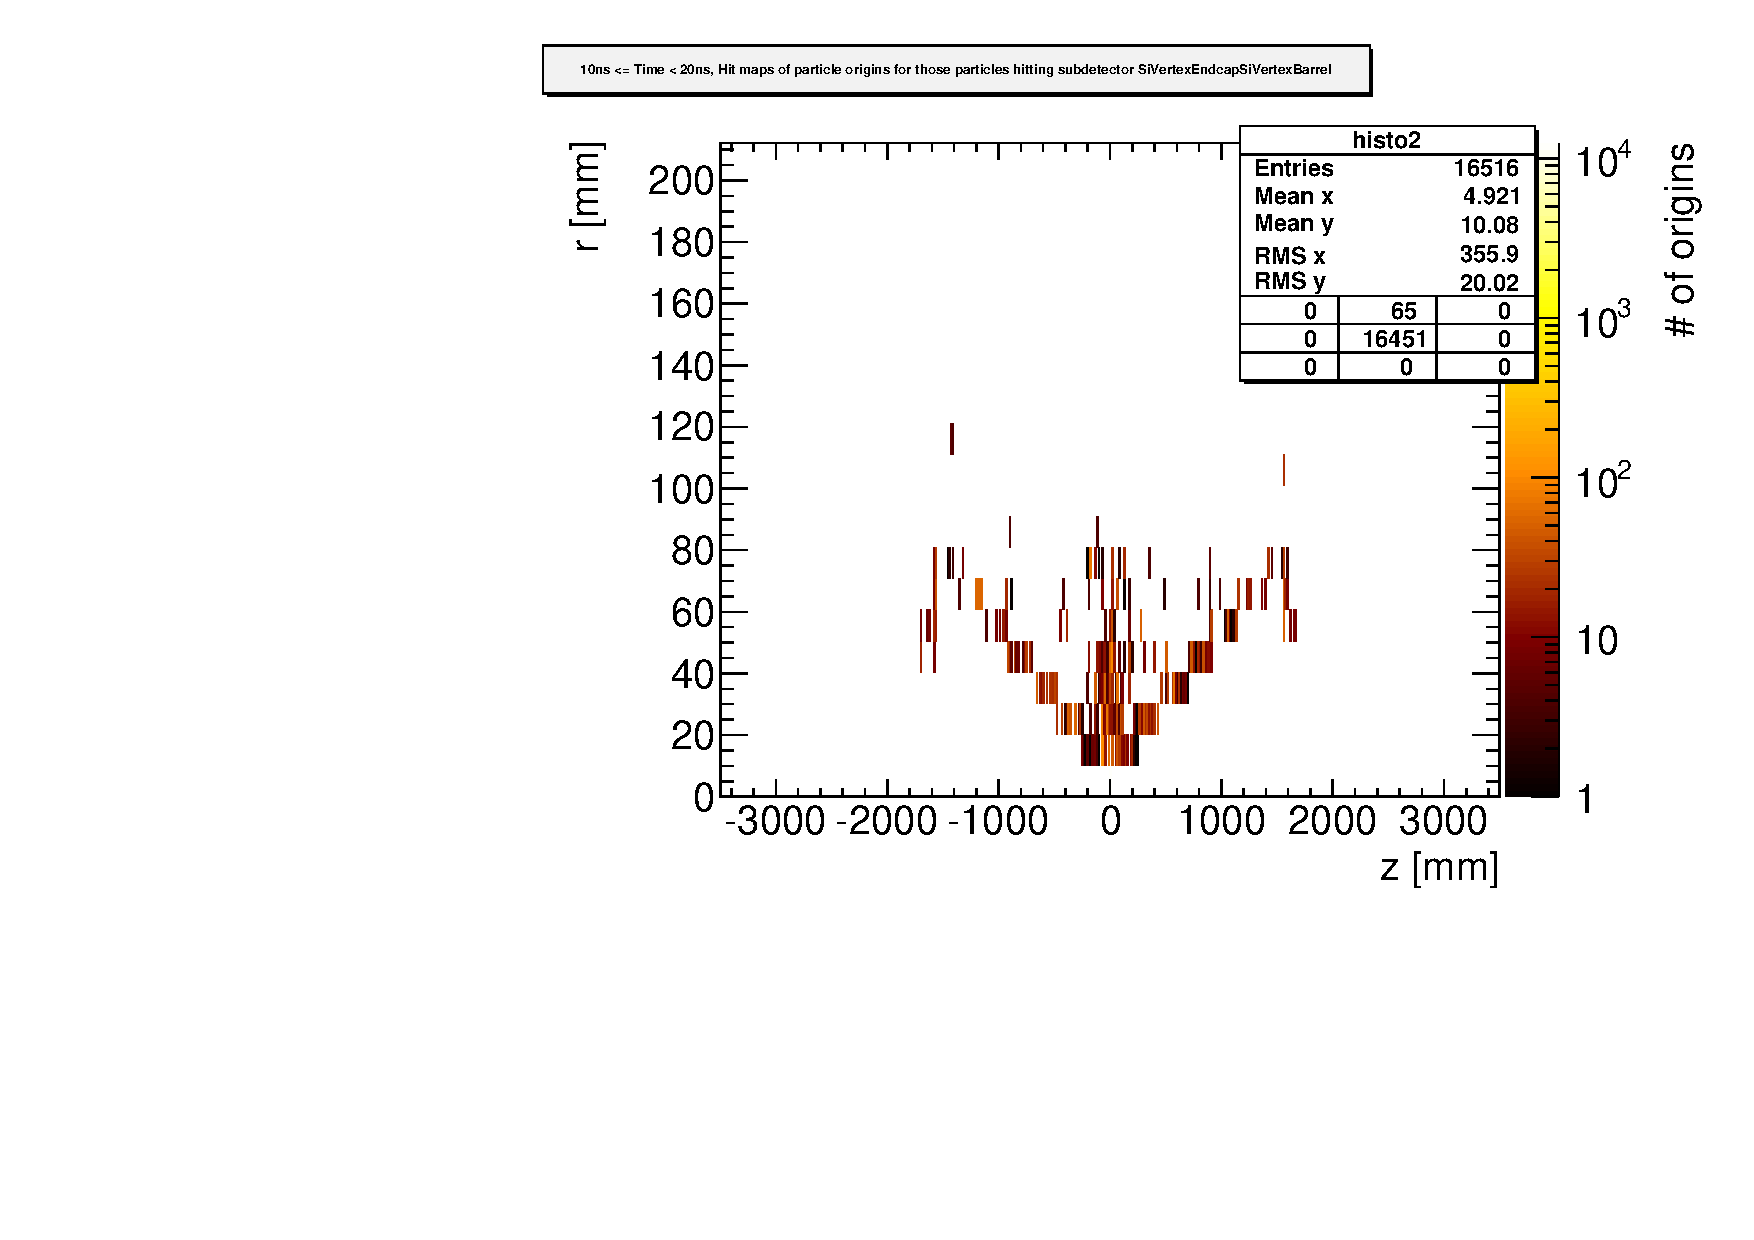
\includegraphics[width=\textwidth]{figures/hitmaps_particleorigins_time2_SiVertexEndcapSiVertexBarrel.pdf}
\caption{$]10\,ns;20\,ns]$.}
\end{subfigure}
%\caption{\footnotesize The radial position as a function of the z-position of the origins of those background particles, that hit the barrel and the endcaps of the vertex detector for $]0\,ns;10\,ns]$, $]10\,ns;20\,ns]$. 1312 bunches are accumulated to increase the statistics.}
\end{figure}
\footnotesize The radial position as a function of the z-position of the origins of those background particles, that hit the barrel and the endcaps of the vertex detector for $]0\,ns;10\,ns]$, $]10\,ns;20\,ns]$. 1312 bunches are accumulated to increase the statistics.
\end{frame}

\begin{frame}{Particle origin of pair bkg particles hitting the vertex detector}
\sidlogo
 \begin{figure}
\begin{subfigure}[t]{0.49\textwidth}
\centering
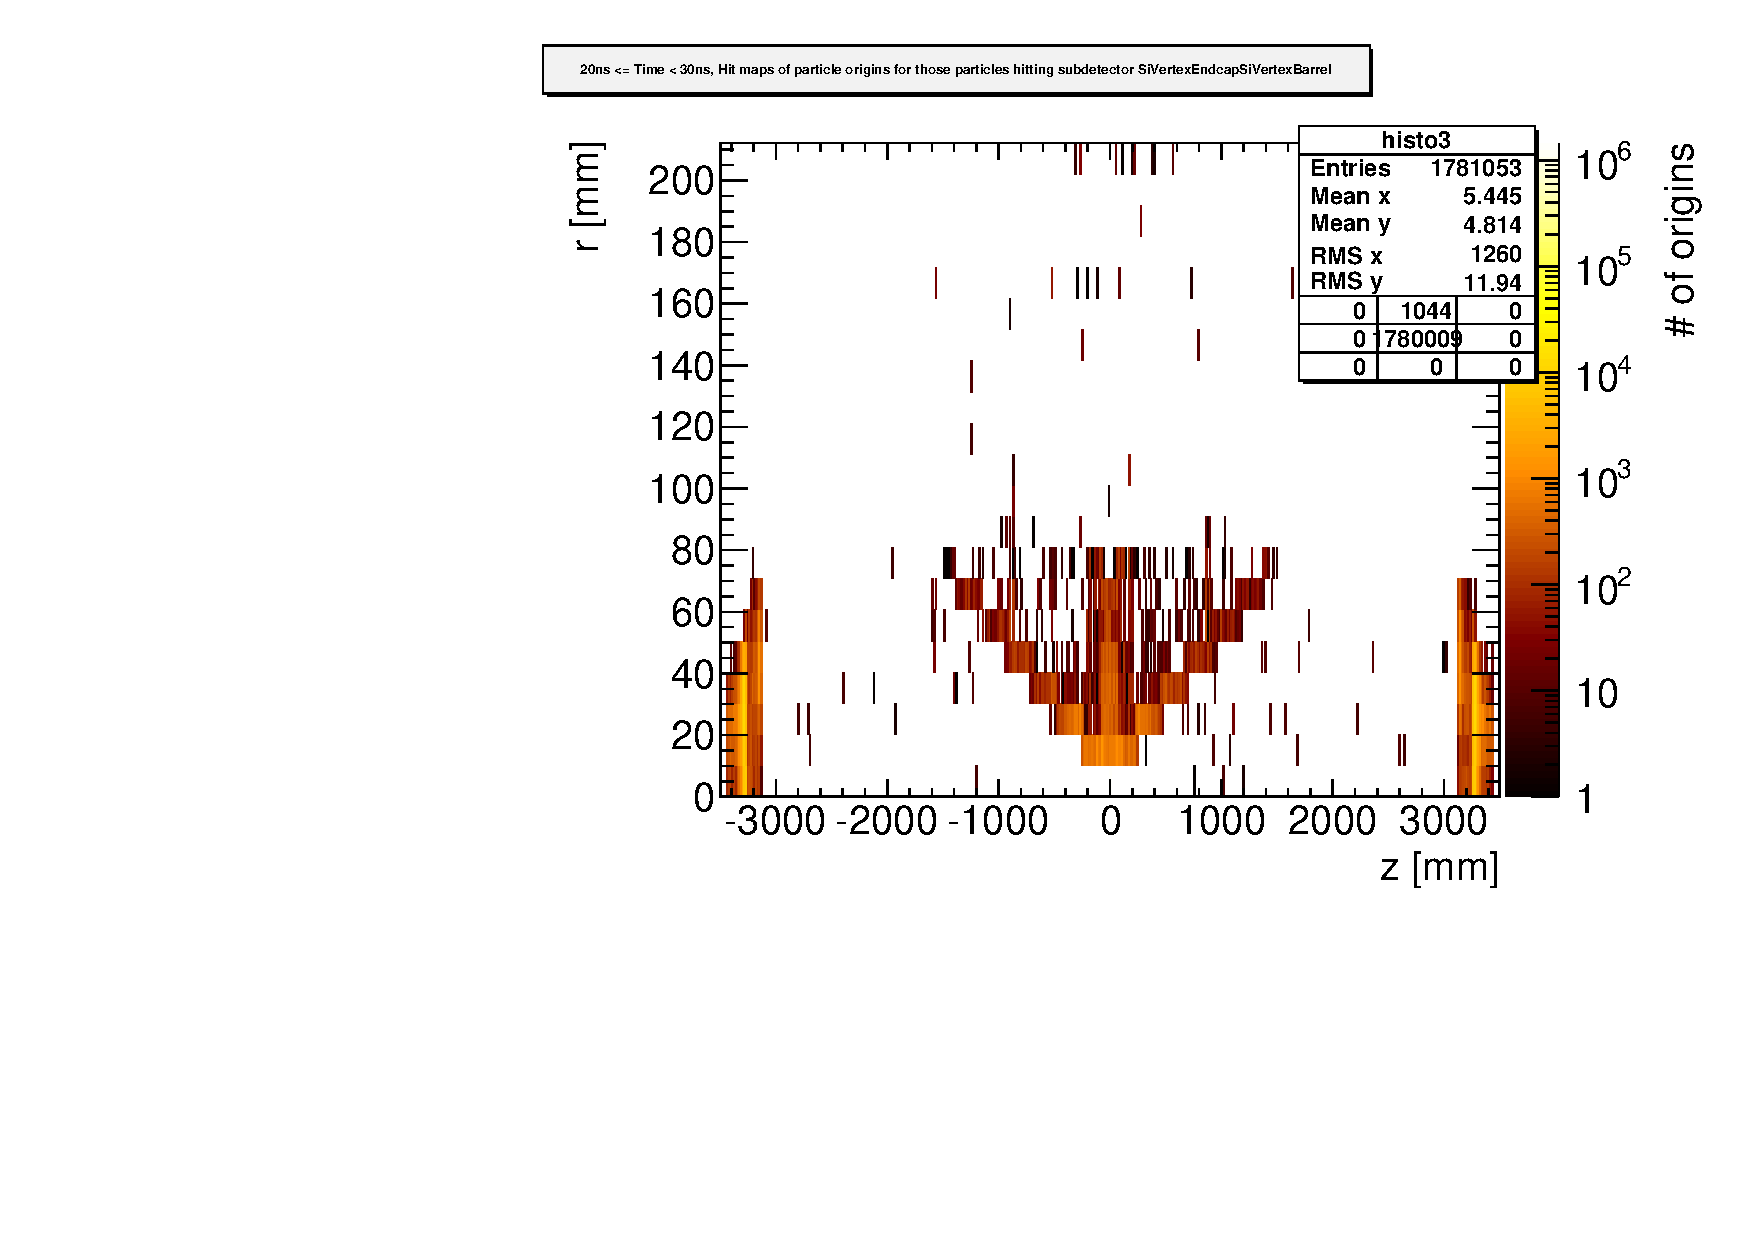
\includegraphics[width=\textwidth]{figures/hitmaps_particleorigins_time3_SiVertexEndcapSiVertexBarrel.pdf}
\caption{$]20\,ns;30\,ns]$.}
\end{subfigure}
\begin{subfigure}[t]{0.49\textwidth}
\centering
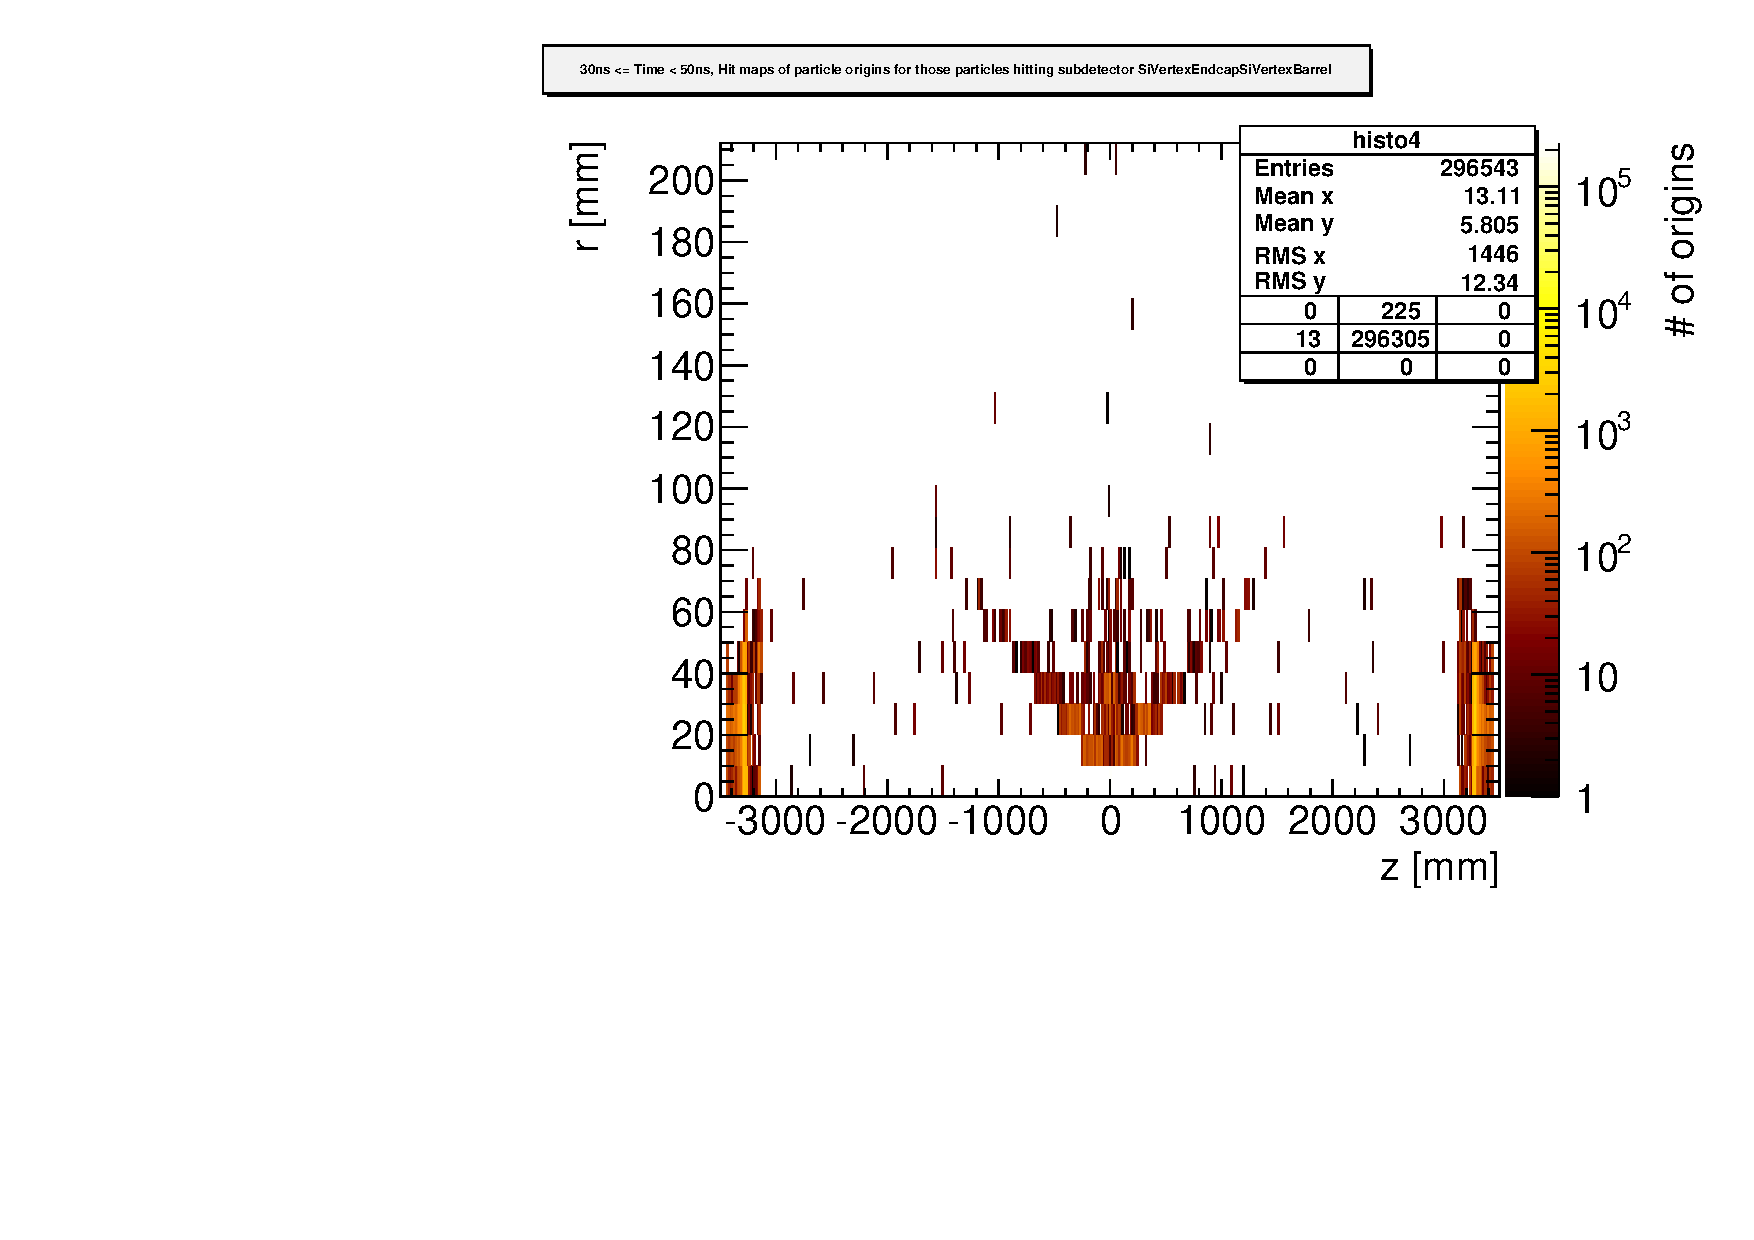
\includegraphics[width=\textwidth]{figures/hitmaps_particleorigins_time4_SiVertexEndcapSiVertexBarrel.pdf}
\caption{$]30\,ns;50\,ns]$.}
\end{subfigure}
%\caption{\footnotesize The radial position as a function of the z-position of the origins of those background particles, that hit the barrel and the endcaps of the vertex detector for $]20\,ns;30\,ns]$ and $]30\,ns;50\,ns]$. 1312 bunches are accumulated to increase the statistics.}
\end{figure}
\footnotesize The radial position as a function of the z-position of the origins of those background particles, that hit the barrel and the endcaps of the vertex detector for $]20\,ns;30\,ns]$ and $]30\,ns;50\,ns]$. 1312 bunches are accumulated to increase the statistics.\\
\normalsize $\Rightarrow$Backscatter particles originate from the endcaps of the SiD detector.
\end{frame}

\section{FLUKA simulation of the ILC Beam Dump}
\begin{frame}
 \begin{center}
  \alert{\MakeUppercase{Neutrons from the beam dump}}
 \end{center}
\end{frame}
{
\usebackgroundtemplate{
 \tikz\node[opacity=0.05]{\includegraphics[width=1.1\paperwidth]{figures/TB-0067-300-00-A_stamp.pdf}};
 }
\begin{frame}{FLUKA simulation of the ILC Beam Dumps}
\flukalogo
The beam is dumped into a water tank after collision.\\Neutrons ($\lesssim$\SI{e10}{\per\square\centi\metre\per\year}) are emitted that radiate the surroundings, and travel back towards the detectors.\\
\vspace*{0.1cm}
Redoing the simulation studies that were done in 2007 (design was not decided back then).
\begin{block}{Simulation step 1}
Implementing the beam dump geometry within FLUKA, using the design drawings by B. Smith~\cite{Smith} to model the dump and the surrounding.
\end{block}

\begin{center}
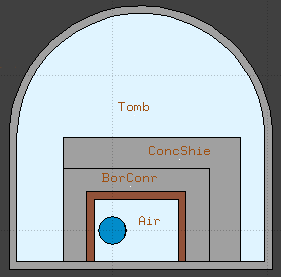
\includegraphics[height=0.35\textheight]{figures/Front_view_BeamDump_Tomb.png}
\hspace*{0.2cm}
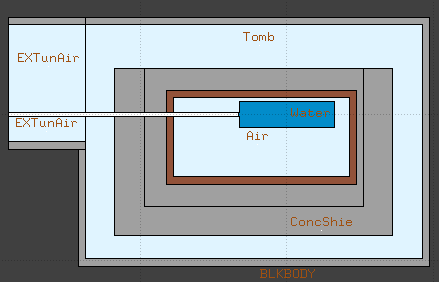
\includegraphics[height=0.35\textheight]{figures/Bird_view_BeamDump_Tomb.png}
\includegraphics[height=0.25\textheight]{figures/done.jpg}
\end{center}
\end{frame}

\begin{frame}{FLUKA simulation of the ILC Beam Dumps}
\flukalogo
\begin{block}{Simulation step 2}
Make FLUKA and FLAIR work, and simulate the neutrons from the beam dumps.
\end{block}

\begin{center}
\includegraphics[width=0.5\textwidth]{figures/NeutronDistribution.png}
\includegraphics[width=0.5\textwidth]{figures/DepositedEnergy.png}\\
\includegraphics[height=0.2\textheight]{figures/done.jpg}
\end{center}
\end{frame}

\begin{frame}{FLUKA simulation of the ILC Beam Dumps}
\flukalogo
\begin{columns}
\begin{column}[c]{0.4\textwidth}
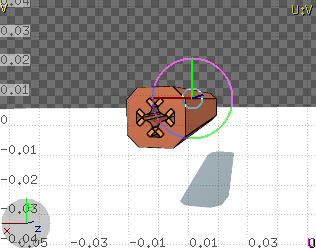
\includegraphics[height=0.45\textheight]{figures/FLUKA_quadrupole_model.png}\\
\small FLUKA simulation model of one of the ILC EXT lattice quadrupoles.
\end{column}
\begin{column}[c]{0.55\textwidth}
\begin{block}{Simulation step 3}
With Benno List (DESY): Python program to plug the real extraction line lattice into FLUKA.\\
Realistic simulation of the interaction between the neutrons and the lattice.
\end{block}
\begin{block}{Simulation step 4}
Simulating the neutrons reaching the interaction point in a full detector simulation.
\end{block}
\end{column}
\end{columns}
\end{frame}

\begin{frame}{Plans for the FLUKA simulation of the ILC Beam Dumps}
 \flukalogo
 All goals of this study in an overview:
\begin{itemize}
 \item Simulating the neutron flux,
 \item the number of neutrons reaching the IP,
 \item the dosis of the surrounding,
 \item the influence of the water composition (amount of deuterium),
 \item the effect of different BeamCal apertures,
 \item the effect of the beam dump design.
\end{itemize}
\end{frame}
}

\section{Final-Focus system as a background source}
\begin{frame}
 \begin{center}
  \alert{\MakeUppercase{Final-Focus system as a background source}\\ \vspace*{0.5cm} Background reduction by Beam Halo collimators}
 \end{center}
\end{frame}

\begin{frame}{Beam Halo Collimators}
\atflogo
\ejadelogo
 \begin{center}
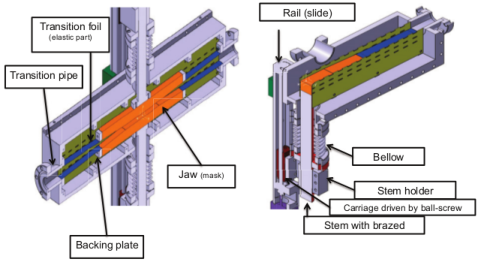
\includegraphics[width=0.5\textwidth]{figures/ATF2_beamhalo_collimator.pdf}
\end{center}

\begin{itemize}
\item In ATF operation time in March: Measured the background level affected by the installed beam halo collimator with Cherenkov detectors
\item Simulating the background with BDSIM (developed by RHUL), after improving the ATF lattice geometry within BDSIM
\end{itemize}
\begin{block}{}
$\Rightarrow$ Studying how much effect a vertical beam halo collimator has on the reduction of the background from the halo interacting with the FF system
\end{block}
\end{frame}

\begin{frame}{Results of the ATF beam operation time}
\atflogo
\ejadelogo
\begin{columns}
 \begin{column}[c]{0.55\textwidth}
 \begin{center}
 \small Cherenkov detector close to the collimator
  \end{center}
 \end{column}
 \begin{column}[c]{0.45\textwidth}
  \begin{center}
 \small Background monitor close to the IP
  \end{center}
 \end{column}
\end{columns}

\begin{columns}
 \begin{column}[b]{0.55\textwidth}
 \begin{center}
   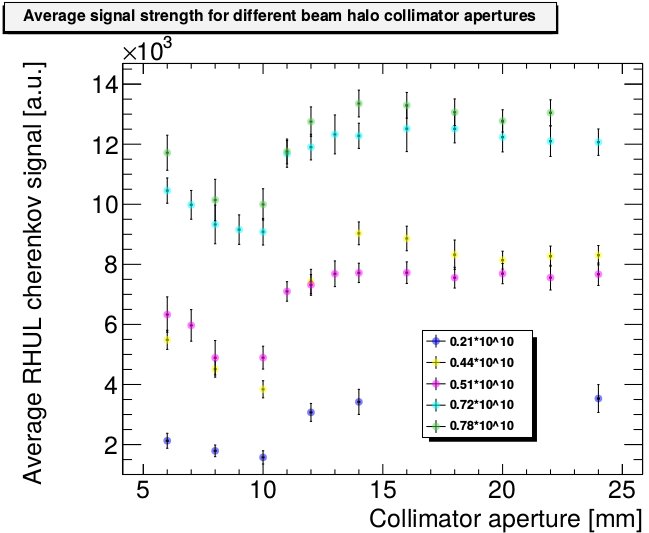
\includegraphics[width=0.9\textwidth]{figures/AverageSignal_perAperture.png}
  \end{center}
 \end{column}
 \begin{column}[b]{0.45\textwidth}
 \flushright
 \tiny [Data taken by Nuria Fuster Martinez (IFIC)]
  \begin{center}
   \includegraphics[width=\textwidth]{figures/Nuria_postIP_Bkg_VerticalCollimator_new_relative.png}
  \end{center}
 \end{column}
\end{columns}
  \flushright{\tiny \alert{See talk by Nuria Fuster Martinez in the ATF session on Wednesday!}}
\begin{block}{}
$\Rightarrow$ Background reduction at the IP of up to 95\%!
\end{block}
\end{frame}

\section{Muons from spoilers}
\begin{frame}
 \begin{center}
  \alert{\MakeUppercase{Muons from spoilers}}
 \end{center}
\end{frame}

\begin{frame}{Muon from spoilers}
 Lewis Keller: MUCARLO simulation of the muon tracks in the BDS tunnel.\\
 \alert{$\Rightarrow$See talk by Glen White in the MDI session of Wednesday:}
 \begin{center}
 	\frame{\includegraphics[width=0.9\textwidth]{figures/Glen_ILC_muons_slide10.pdf}}
  \end{center}
\end{frame}
\begin{frame}{Muons at IP}
\small [Glen White, Lewis Keller (SLAC)]
  \begin{center}
 	\frame{\includegraphics[width=0.8\textwidth]{figures/Glen_ILC_muons_slide12.pdf}}
  \end{center}
\end{frame}
\begin{frame}{Muons at IP}
\small [Glen White, Lewis Keller (SLAC)]
  \begin{center}
 	\frame{\includegraphics[width=0.9\textwidth]{figures/Glen_ILC_muons_slide11.pdf}}
  \end{center}
\end{frame}


\section*{Summary}
\begin{frame}{Summary}
Current effort in simulating the background at the IP:
 \begin{itemize}
  \item Background from beam-beam interactions
    \begin{itemize}
      \item Pair background, bhabha scattering and \textgamma\textgamma$\rightarrow$hadrons
      \item Occupancy studies in the SiD detector
      \item Hit time studies
    \end{itemize}
  \item Neutron background from the main beam dump
      \begin{itemize}
      \item FLUKA simulation of the neutrons emitted
      \item Studies of different beam dump designs
      \item Studies of the doses of the surroundings
    \end{itemize}
  \item Background from the Final-Focus system
    \begin{itemize}
      \item Performance studies of a vertical beam halo collimator at ATF2
      \item BDSIM simulations of the relative beam background reduction by beam halo collimations
    \end{itemize}
  \item Muon background from spoilers
  \begin{itemize}
   \item Studies of the SiD detector occupancies by muons are needed
  \end{itemize}

 \end{itemize}
 
 
\end{frame}




\section*{The end}
{
\usebackgroundtemplate{
 \tikz\node[opacity=0.1]{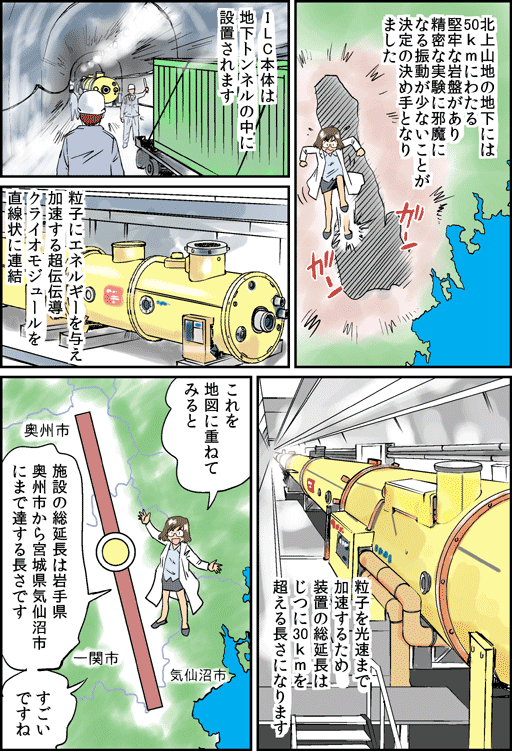
\includegraphics[width=\paperwidth,resolution=200]{figures/ilc-Comic.png}};
 % \tikz\node[opacity=0.2]{\centering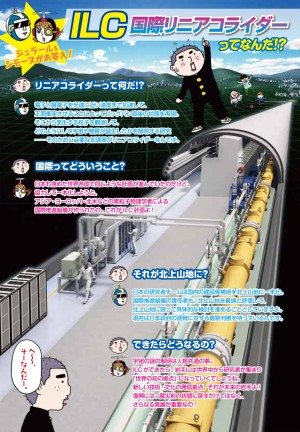
\includegraphics[height=\paperheight]{figures/Iwatecomics.jpg}};
 }
\begin{frame}
\ilclogo
\begin{center}
\textcolor{RubineRed}{
	\LARGE Thanks!\\
	%\vspace*{0.5cm}
	%\begin{CJK}{UTF8}{min}
	%どうもありがとうございます。
	%\end{CJK}
}
\end{center}
\end{frame}
}

\section*{References}
\begin{frame}{References}
\begin{thebibliography}{9}
\setbeamertemplate{bibliography item}[text]

\bibitem{Grid} /ilc/user/a/aschuetz/GuineaPig
\bibitem{Jan_Grid} /pnfs/desy.de/ilc/user/j/jstrube
\bibitem{TDR} T. Behnke, et al. \emph{The International Linear Collider - Technical Design Report}, 2013.
\bibitem{Smith} B. Smith (Rutherford Lab), \emph{Design drawings 0-TB-0067-300-00-A, 0-TB-0067-210-00-A, 0-TB-0067-404-00-A}, Dec. 2006 - Jan. 2007.
\bibitem{Collimator} N. Fuster-Martínez, IFIC (CSIC-UV), et al. \emph{Design study and construction of a transverse Beam Halo Collimation system for ATF2}, 2015. \url{http://accelconf.web.cern.ch/AccelConf/IPAC2015/papers/wepmn059.pdf}
\bibitem{Muons} MUCARLO simulations: Lewis Keller (SLAC)

\end{thebibliography}
\end{frame}


%--------------------------------------------------------------------------------
\section{Appendix}
\appendix

\begin{frame}
\begin{center}
\LARGE Additional Material
\end{center}
  \tableofcontents
\end{frame}

\section{Background simulations}
\subsection{GuineaPig}
\begin{frame}{GuineaPig data}
Accelerator parameters needed as input to GuineaPig are available for different ILC modes.\\
Already simulated pair background files for >3900 bunches are on the Grid as service to the community.\cite{Grid}\\
\visible<2->{
One bunch has about 200,000 background particles:
 \begin{figure}
 	\begin{columns}
        \column[T]{0.75\linewidth} 
        \begin{flushright}
        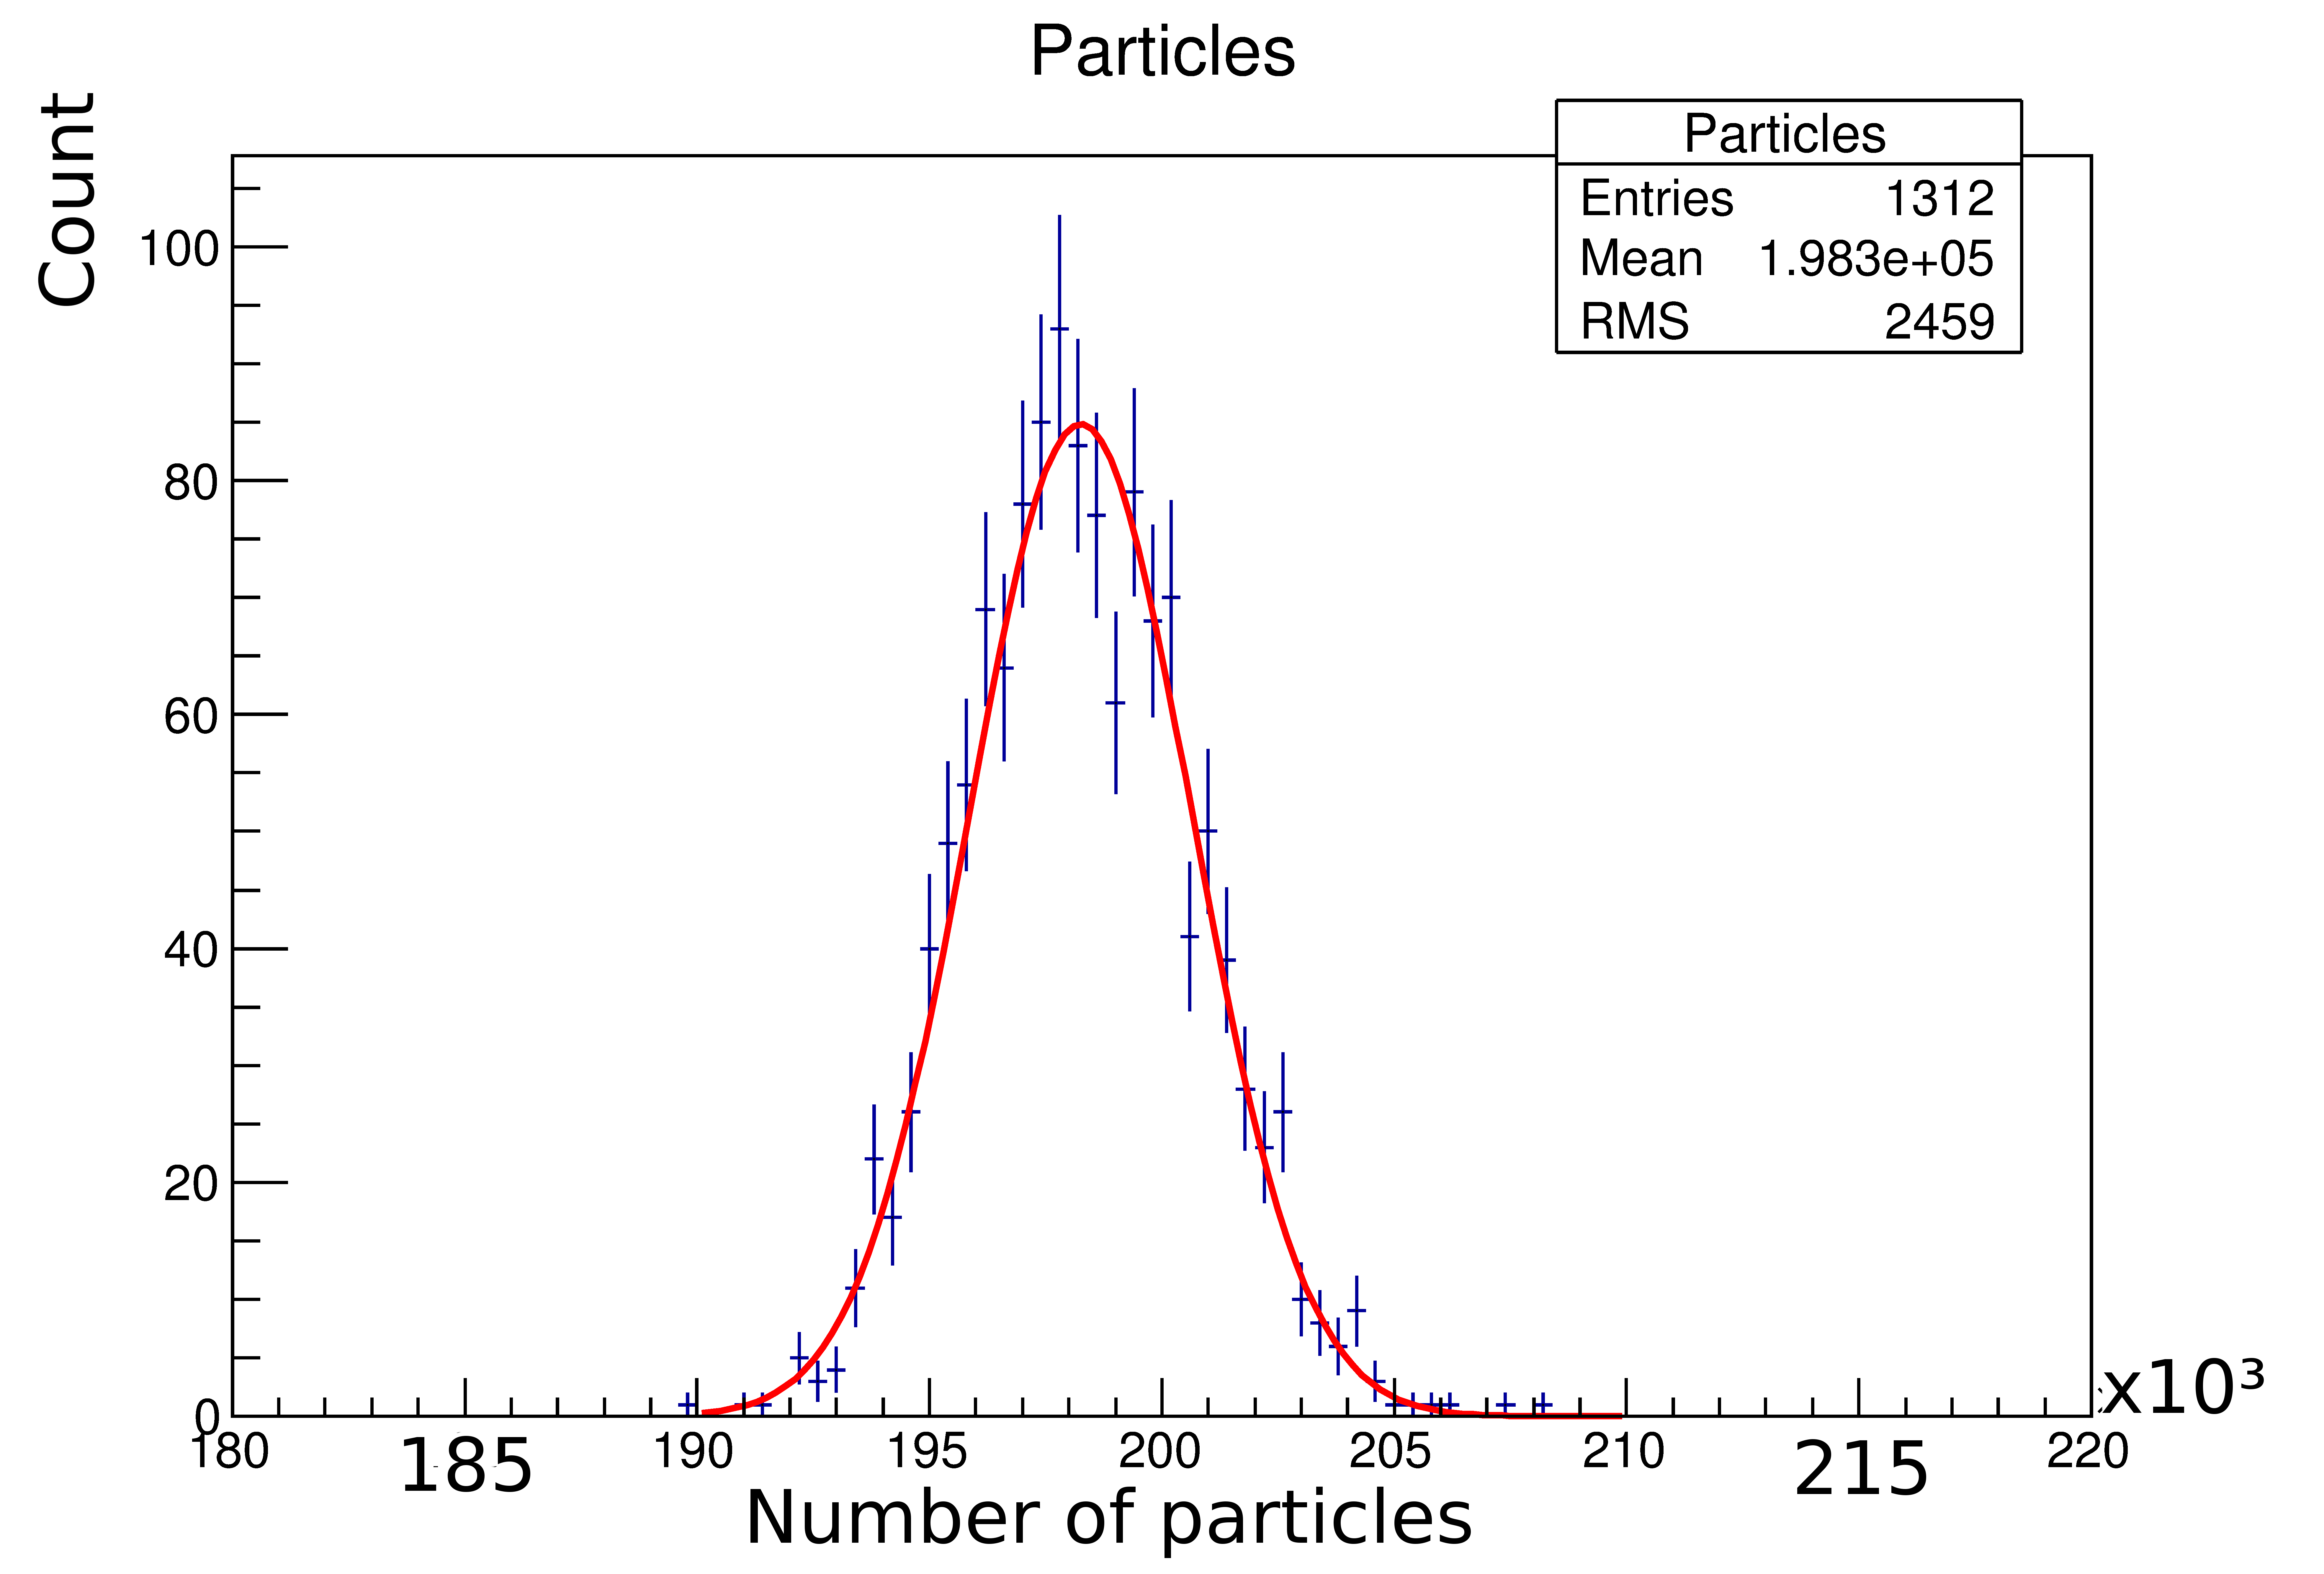
\includegraphics[height=0.55\textheight]{figures/sidloi3_pairs_1312_EcalEndcap_HitsPerFile_Particles.png}
        \end{flushright}
        \column[T]{0.25\linewidth}
        \begin{flushleft}
        \caption{\small Distribution of number of pair background particles per bunch in a train of 1312.}
        \end{flushleft}
      \end{columns}
\end{figure}
}
\end{frame}

\subsection{Occupancy studies}
\begin{frame}{Vertex detector barrel and endcaps - all bkg}
Occupancy distributions in the single layers of the vertex barrel and endcaps:
\includegraphics[width=0.52\textwidth]{figures/VX_occ_barrel.png}
\includegraphics[width=0.52\textwidth]{figures/VX_occ_endcap.png}
\end{frame}

\subsection{Hit time distributions}
\begin{frame}{Vertex detector barrel and endcaps - Pair bkg}
Hit time distributions of the first bunch of pair background in the vertex barrel and endcaps:
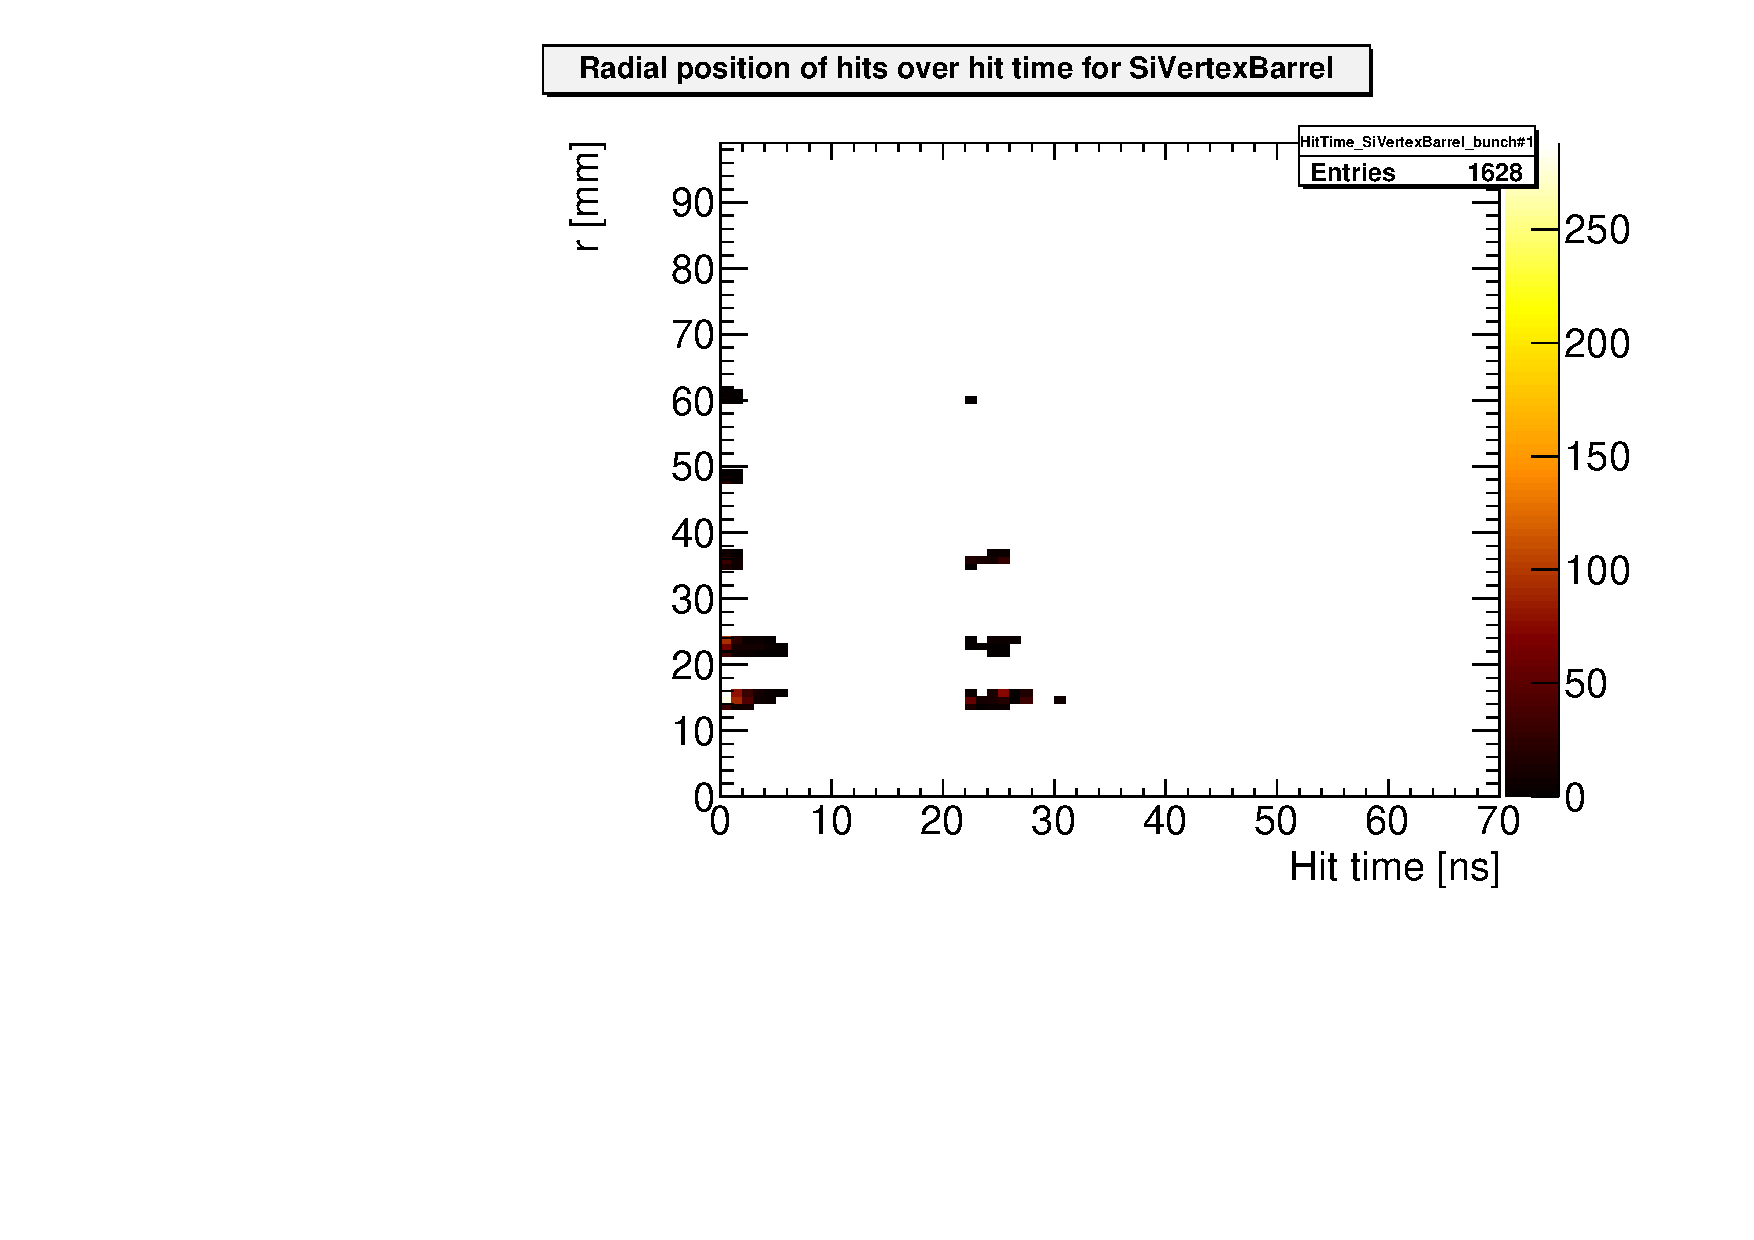
\includegraphics[width=0.52\textwidth]{figures/hittime_SiVertexBarrel_IRrealign_1bunch.pdf}
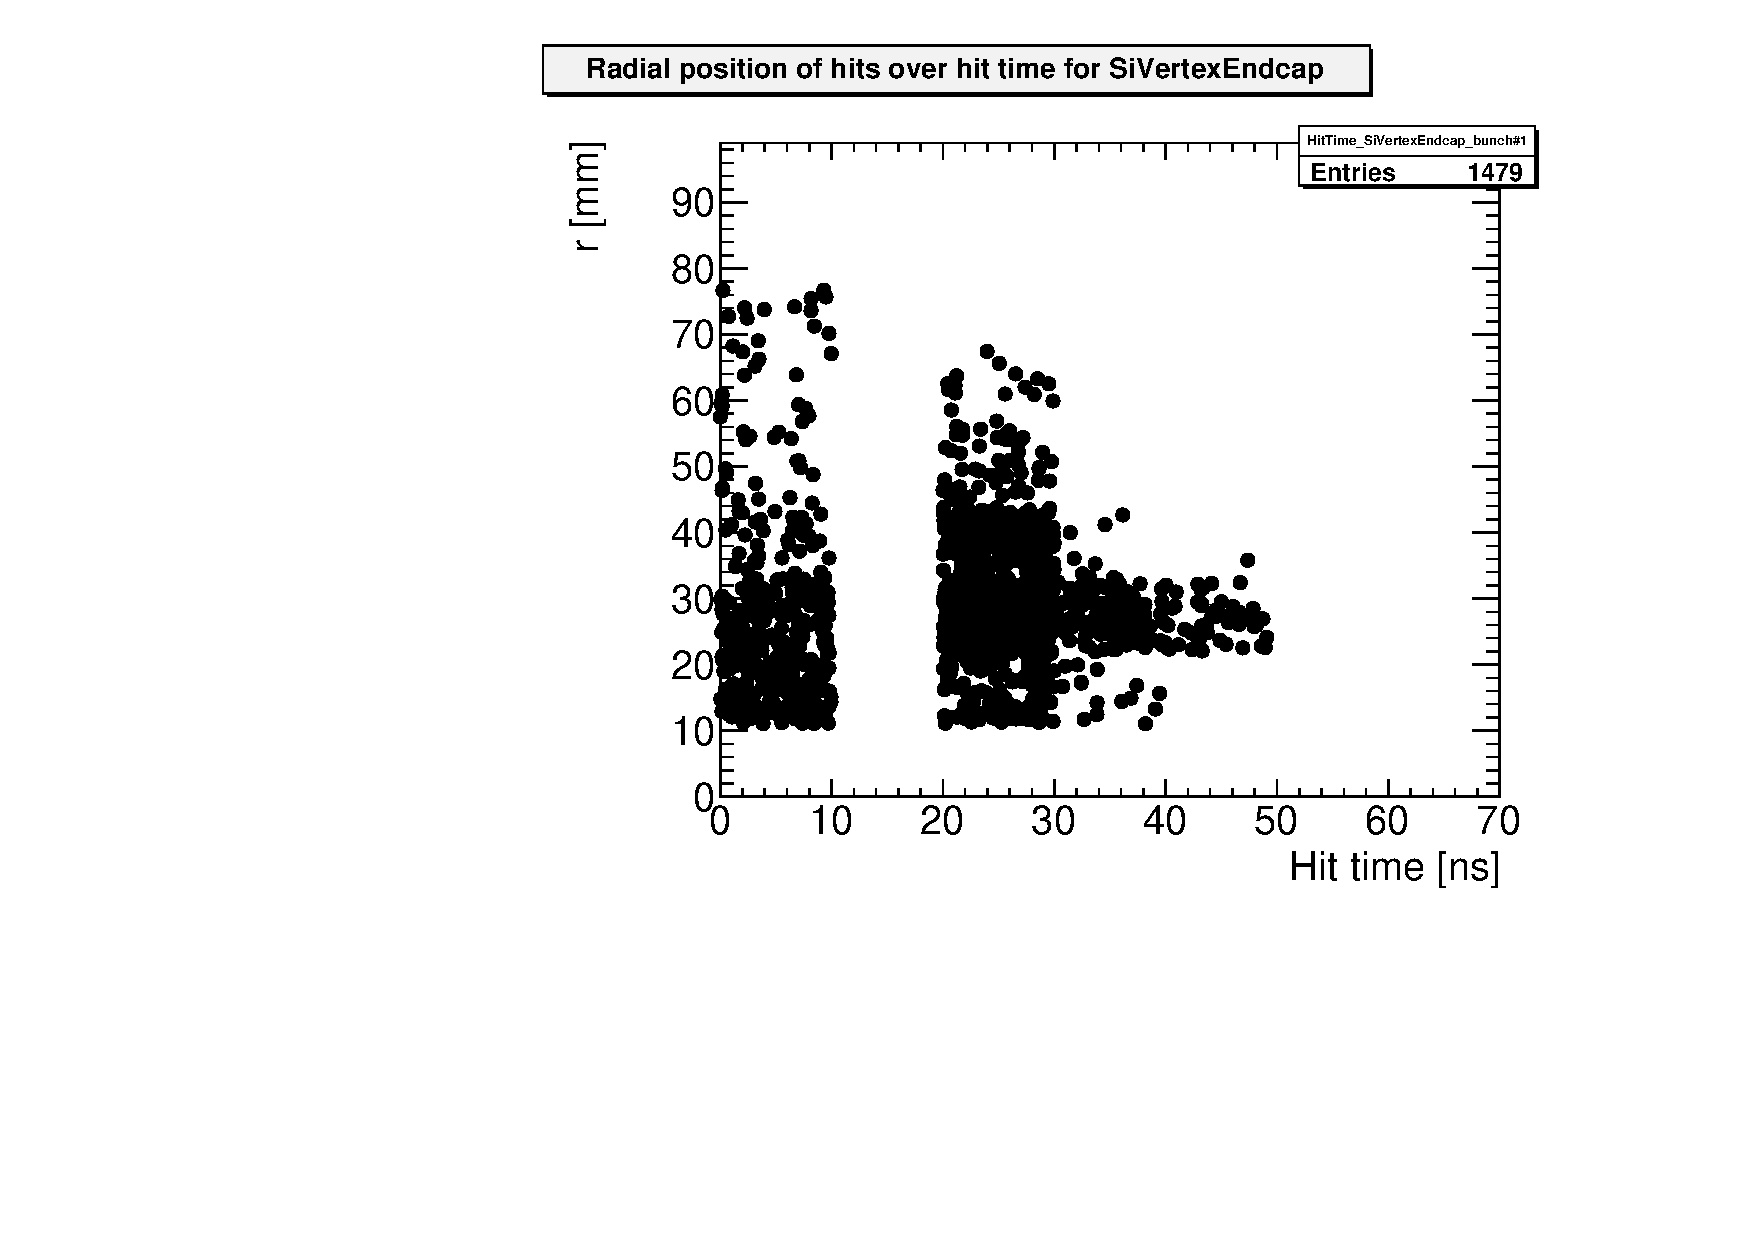
\includegraphics[width=0.52\textwidth]{figures/hittime_SiVertexEndcap_IRrealign_1bunch.pdf}
\end{frame}

\section{BDSIM}
\begin{frame}{BDSIM}
\rhullogo
BDSIM is:
\begin{itemize}
 \item a Geant4 extension toolkit for the simulation of particle transport in accelerator beamlines
 \item developed at RHUL
\end{itemize}
 \begin{center}
 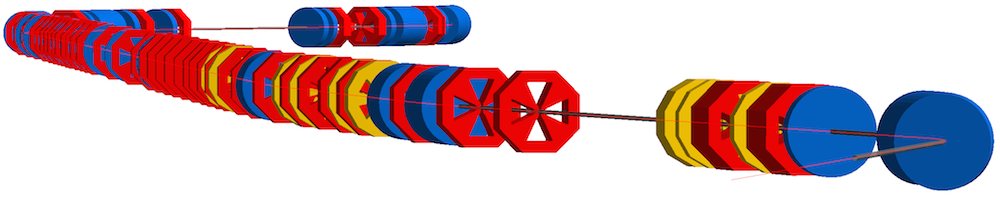
\includegraphics[width=0.5\textwidth]{figures/atf_bdsim.png}
\end{center}
Accelerator descriptions from other tools such as MADX can be converted to BDSIM input.
\begin{columns}
 \begin{column}[b]{0.35\textwidth}
  \centering
   \includegraphics[width=0.5\textwidth]{figures/Flange_+z_view2.jpg}\\
   \tiny New GDML geometry visualization of a beam pipe flange between a rectangular and a circular beam
pipe at the location of the Cherenkov detector.
 \end{column}
 \begin{column}[b]{0.65\textwidth}
   Current simulation status:
\begin{itemize}
 \item Improving the ATF lattice geometry within BDSIM in the region of the collimator
 \item Updating the BDSIM source code regarding these changes
\end{itemize}
 \end{column}
\end{columns}
\end{frame}

\section{Beam dump study}
\begin{frame}{Beam dump tank drawing - Jan 2007}
 \includegraphics[width=\textwidth]{figures/TB-0067-210-00-A_stamp.pdf}
\end{frame}
\begin{frame}{Beam dump tank drawing - Jan 2007}
 \includegraphics[width=\textwidth]{figures/TB-0067-300-00-A_stamp.pdf}
\end{frame}
\begin{frame}{Beam dump building drawing - Dec 2006}
 \includegraphics[width=0.65\textwidth,angle=90]{figures/0067_404__2__Layout1__1__stamp.pdf}
\end{frame}

\end{document}
